\documentclass[12pt,fleqn]{article}\usepackage{../../common}
\begin{document}
Ders 3

Bugünkü dersin konusu dış dünyayı modellemek, kamera hareketini temsil
edebilmek, bu sırada Lie grupları, Lie cebirini de öğreneceğiz. Lie grubu,
adı üstünde bir grup, fakat ek olarak bazı ek tanımlar içeriyor. Örnek
olarak kamera hareketi bir Lie grubu oluşturuyor. Kamera transformasyonunun
(hareketinin) tersi alınabilir, ki genel Lie grupları için de bu mümkün,
tabii bu fiziksel kamera hareketi için de doğru, kameraya başlattığımız
noktaya geri getirebiliriz. Ama esas önemli nokta şu: kameranın hareketini
sürekli bir ortamda tanımlamak mümkün - sonsuz küçüklükteki (infinitesimal)
kamera hareketleri tanımlanabilir, ki bu durum kamera hareketini Lie grubu
yapan en önemli faktör.

Üç Boyutlu Öklit Uzayı

Üç boyutlu Öklit uzayı $\mathbb{E}^3$, tüm $p \in \mathbb{E}^3$ noktalarından oluşur, ki bu noktalar

$$ X = \left[\begin{array}{ccc} X_1,X_2,X_3 \end{array}\right]^T \in \mathbb{R}^3$$

kordinatları ile karakterize edilir. $\mathbb{E}^3$ ve $\mathbb{R}^3$ aynı
olarak kabul edilebilir. 

Eldeki iki nokta $X,Y$ için

$$ v = Y - X \in \mathbb{R}^3$$

Bir vektör elde ettik, ki bu vektör (diğer tüm vektörler gibi) başlangıç
noktasından bağımsız. $\mathbb{R}^3$ içindeki tüm vektörler bir lineer
vektör uzayı oluşturur. $\mathbb{E}^3$'u $\mathbb{R}^3$ ile eş kabul ettik,
o zaman $\mathbb{R}^3$'den tek sayı çarpımı, norm, ölçekler gibi
özellikleri alabiliriz, bu sayede uzaklıkları, ya da eğri uzunluğu gibi
şeyleri hesaplayabiliriz, mesela 

$$ I(\gamma) = \int_{0}^{1} | \dot{\gamma}(s)| \ud s $$

ki bu herhangi bir $\gamma: [0,1] \to \mathbb{R}^3$ eğrisi için. Formüldeki $||$
bir Öklitsel norm, $\mathbb{R}^3$'ten geliyor.

Çapraz çarpımı görmüştük.

Tüm $3 \times 3$ eksi bakışımlı matrislerin uzayı so(3) olarak gösterilir,
dikkat daha önce SO(3) vardı, özel dikgen matrislerin uzayı. Bu so(3),
küçük harfli olan, farklı. Ne şekilde onu birazdan göreceğiz. Aradaki
bağlantıyı hemen belirtebilirim ama, SO(3) bir Lie grup, so(3) onunla
ilişkili olan Lie cebiri. 

Daha önce katı gövde transformasyonundan bahsettik, ve kamera hareketi
böyledir dedik; yani yer değişimi + rotasyon. Fakat katı gövde hareketini
tanıştırmanın bir değişik yolu daha var, hatta bu yol katı gövde
tanımındaki ``katı'' kelimesine daha uygun, bu tanıma göre bir objenin
üzerinde iki nokta düşünelim, bu iki nokta arasındaki mesafe transformasyon
ardından değişmeden kalmalı. İşte bu sebeple gövde ``katı'' çünkü
değişmiyor. Formel olarak belirtmek gerekirse katı gövde transformasyonları
su aileye

$$ g_t: \mathbb{R}^3 \to \mathbb{R}^3; \qquad X \to g_t(X), \qquad t \in [0,T] $$

ait olan eşlemelerdir (yani fonksiyonlardır) öyle ki herhangi iki vektörün
norm ve çapraz çarpımı muhafaza edilir,

$$ |g_t(v)| = |v|, \quad \forall v \in \mathbb{R}^3 $$

$$ g_t(u) \times g_t(v) = g_t(u \times v), \quad \forall u,v \in \mathbb{R}^3 $$

Üstteki tanım aynı zamanda noktasal çarpımın da değişmediği anlamına
geliyor, bu üstteki tanımdan bariz olmayabilir, ama norm ve tek sayı
çarpımı kutupsal özdeşlik (polarization identity) üzerinden norm ile
alakalı olduğu için, 

$$ \langle u,v \rangle = \frac{1}{4} ( |u+v|^2 - |u-v|^2 ) $$

o zaman noktasal çarpımın da değişmemesi gerekir. 

Daha bitmedi: eğer üstteki üç tanım doğru ise o zaman üçlü çarpım (triple
product) da muhafaza edilir demektir, ki $\forall u,v,w \in \mathbb{R}^3$ için

$$ \langle g_t(u), g_t(v) \times g_t(w) \rangle = \langle u, v\times w \rangle  $$

eşitliği doğru olmalıdır. Bu ifade aynı zamanda katı gövde transformasyonun
``hacmi muhafaza ettiği'' anlamına da gelir, çünkü üstteki ifade hacim
hesabı için kullanılır. Lise matematiğinden hatırlanacağı üzere,

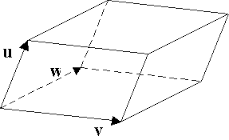
\includegraphics[height=3cm]{volume.png}

üç vektörün kapsadığı hacmin hesabı üstteki formüldür. Yani katı gövde
hareketi üçlü çarpımı muhafaza ediliyor demek, bu da hacmi muhafaza ediyor
demektir. Bazı hareketler vardır ki katı gövde değildir, mesela bir süngeri
alıyorum, sıkıştırıyorum, bu hareket hacmi muhafaza etmedi.

Peki üstteki tanım katı gövde hareketini kesinlikle temsil eder mi? Bunu
formel bir şekilde göstermek istiyoruz; transformasyon $g_t$, ki $t$
anındaki katı gövde değişimini gösteriyor. Bu ispat için değişimin bir
orijin ve 3 tane birimdik (orthonormal) vektör $e_1,e_2,e_3 \in
\mathbb{R}^3$'u nasıl etkilediğini göstermem yeterli. Diğer her nokta bu
baza referanslı olacağı için bu yeterli oluyor. Orijinin hareketini yer
değişimi $T \in \mathbb{R}^3$ olarak göstereyim, vektör $e_i$'ların
transformasyonu ise $r_i = g_t(e_i)$, bu transformasyon sonrası yeni bir
baz elde etmiş olacağız.

Tek sayı ve çapraz çarpımı muhafaza edilir demiştik, yani

$$ r_i^Tr_j = g_t(e_i)^Tg_t(e_j) =
e_i^Te_j = \delta_{ij}, 
\qquad r_1 \times r_2 = r_3
$$

$\delta_{ij}$ hatırlarsak $i=j$ ise 1, değil ise 0 veren bir notasyonel ifade. 

Üstteki 1. kısıtlama matris $R = \left[\begin{array}{ccc} r_1&r_2&r_3 \end{array}\right]^T$ 
dikgen (rotasyon) matrisi demek ile aynı şeydir, yani $R^TR = RR^T = I$. Ve
çapraz  çarpımlı 2. ifade $\det(R) = +1$  demektir, yani $R$ matrisi, 

$$SO(3) = \{ R \in \mathbb{R}^{3 \times 3} \mid R^TR = I, \det(R) = +1\}$$

grubunun bir üyesidir. Ve evet, katı gövde hareketi hakikaten de 

$$ g_t(x) = Rx + T $$

olarak yazılabilir.

Rotasyon matrisine yakında bakalım. Dediğimiz gibi bir açı üzerinden
rotasyon yapabiliriz, ve tüm bu rotasyonlar bir grup oluşturur. Sonsuz
küçük rotasyon da mümkündür, kamerayı alırım, azıcık döndürürüm. Bu
döndürme gruptaki bir öğeye tekabül eder. Bu her türlü grup için geçerli
olmayabilir, mesela içinde yine sonsuz tane öğe olan tam sayıları alsam,
azıcık değişimi bu küme içinde temsil edemezdim, çünkü öğeler ayrıksal
(discrete). 

Niye sonsuz küçüklükteki rotasyonlara bakıyoruz?  Rotasyonları temsil etmek
aslında külfetli bir iş; mesela rotasyonların olduğu uzay lineer değil, iki
rotasyon matrisi $R,\tilde{R}$'yi alsam mesela ve onları toplasam (ki
böylece bir toplam döndürmeyi hesaplayacağımı umardım) yeni bir rotasyon
matrisi elde edemiyorum. Zorluk aslında $R^TR=I$ ve $\det(R)=+1$
kısıtlamalarından ileri geliyor. Mesela iki resim var, bu resme bakarım bir
kameranın nasıl döndüğünü göstermek istiyorum, rotasyon matrisi şöyle
olacak,

$$ 
\left[\begin{array}{rrr}
a & b & c \\ d & e & f \\ g & h & i
\end{array}\right]
 $$

Bu matristeki değişkenlerin değerini atamakta serbest olamıyorum,
dediğim gibi, belirtilen iki kısıtlamaya uymam lazım. Yani bir optimizasyon
işletip üstteki 9 değişkeni hesaplamaya uğraşırken bir de onun üstüne 2
tane çok ağır şarta da uymam lazım. Bu şartlardan en ağırı determinant
aslında. 

O zaman sonsuz küçüklükteki rotasyonun temsilini türetelim; bir rotasyon
ailesini temsil eden $R(t)$ olsun, ki bir noktayı sürekli transform
ediyorlar, başlangıç noktası $R(0) = I$, yani birim matrisi,

$$ X_{trans}(t) = R(t) X_{orig}, \qquad R(t) \in SO(3) $$

Bir $X_{orig}$ noktasını aldım, ve her $t$ anında döndürüyorum, sonuç
$X_{trans}$. Tabii noktanın yeri değişmiyor, ama kameranın ekseni değiştiği
için ona göre nokta değişmiş gibi oluyor. 

$R(t)R(t)^T = I$, $\forall t$ olduğu için (olmalı çünkü rotasyon matrisleri
dikgen) bu aynı anda, her $t$ anı için bu çarpımın sabit olduğu sonucunu
verir, ve her $t$ için sabit olan bir şeyin, Analiz dersinden
hatırlayabileceğimiz üzere, $t$'ye göre türevi sıfır olmalıdır. Yani,

$$ \frac{d}{dt} (RR^T) = \dot{R}R^T + R \dot{R}^T = 0 $$

$$  \dot{R}R^T = - (\dot{R}R^T)^T  $$

Bu bize $\dot{R}R^T$'nin eksi bakışımlı matris olması gerektiğini söylüyor,
yani önceden $\land$ operatörü ile ulaştığımız bir sonuç noktası. O sonuç
noktasına $\hat{w}(t)$ diyelim,

$$\dot{R}(t)R^T(t) = \hat{w}(t)$$

Sağdan $R(t)$ ile çarpalım, 

$$\dot{R}(t) = \hat{w}(t)R(t)$$

$R(0)=I$ olduğuna göre, üstte yerine koyalım, 

$$\dot{R}(0) = \hat{w}(0)  $$

Bu demektir ki eksi bakışımlı matris $\hat{w}(0) \in so(3)$ bize birim
matris $I$ etrafında rotasyon için 1. derece bir yaklaşıksallık sağlıyor,
yani 

$$ R(dt) = R(0) + dR = I +  \hat{w}(0) dt $$

Yani rotasyonu bir teğet uzayında harekete çevirmiş oldum. Bu uzaya Lie
cebiri ismi veriliyor. Elde ettiğim avantaj bir teğet uzayının,
$\hat{w}(0)$ yönünde, daha rahat işlem yapabilmeme izin vermesi. Bu uzayın
öğeleri eksi bakışımlı matrisler, yani köşegenleri sıfır, bazı öğeleri
dolu, vs. ve serbestlik derecesi 3 olan rotasyon bir uzay bu. Eğer
rotasyonları 9 öğesi dolu olan bir matris, onun üstüne iki tane kısıtlama
üzerinden tanımlasaydım, işler arap saçına dönecekti. Eksi bakışımlı
matrisler üzerinde işlemler çok daha rahat oldu.

Kamera hareketinin kestirilmesi / hesaplanması için yapılan budur; Lie
cebiri içinde, o lineer uzayda kalarak bir hesap yapmak böylece kamera
hareketini yaklaşıksal olarak bulmak. Bunu sadece 3 serbestlik derecesi
üzerinden yapabilirim, başka hiçbir kısıtlamaya bakmam
gerekmez. Kısıtlamaları dikkate alarak yapılması gereken optimizasyon çok
saç yolduracak bir iştir. Bundan mümkün olduğunca kaçınmak gerekir.

Üstte yaptıklarımız işin ruhu olarak şuna da benzeyebilir: Mesela rotasyon
şu şekilde de gösterilebilir,

$$ 
\left[\begin{array}{rrr}
\cos \theta & -\sin \theta \\
\sin \theta & \cos \theta 
\end{array}\right]
 $$

$\theta=0$ dersem birim matrisi elde ederim. Şimdi diyelim ki sıfır değil
ama ``sıfıra çok yakın'' bir değerim var; matristeki terimler için bir
Taylor açılımı yapabilirim, ve 1. derece terimleri kullanırsam,

$$ 
\left[\begin{array}{rr}
\theta & 0 \\ 0 & \theta 
\end{array}\right]
 $$

elde ederim, ki bu matris bir eksi bakışımlı matristir, birim matris artı
üstteki değişime geldik. Ama tabii tek düzlemde olunca zaten tek serbestlik
derecesi var, $\theta$. Ama üç boyutlu rotasyon söz konusu olunca ifade
üstteki kadar temiz olmuyor, ki Lie cebirine vs. bunun için giriyoruz. 

Ana konumuza dönelim; Tüm rotasyonlar Lie grubu, teğet uzayı Lie
cebiri. Gösterdik ki sonsuz küçük bir dönüş $R \in SO(3)$'un etkisi, eksi
bakışımlı matrisler uzayının

$$ so(3) = \{ \hat{w} \mid  w \in  \mathbb{R}^3\} $$

bir öğesi ile yaklaşıksal olarak temsil edilebilir. Bu rotasyon grubu SO(3)
Lie grubudur, so(3) ise Lie cebiridir. 

Tanım

Bir Lie grup (ya da sonsuz ufak grup) aynı anda hem grup hem de bir pürüzsüz
bükümdür (smooth manifold). Grup operasyonları çarpma ve tersini alma bir
pürüzsüz eşlemedir (smooth maps). Gösterdik ki birim matris noktasında rotasyon
grubu SO(3)'un teğeti so(3) Lie cebiri.

Pek çok değişik Lie grubu vardır, ama bilimde en yaygın kullanılanı
SO(3). Ayrıca yer değiştirme için gereken SE(3) grubu (özel Öklitsel grup).

Bu arada ``cebir'' kelimesi kafa karıştırmasın; burada cebir kelimesinin
soyut matematikteki anlamını kullanıyoruz, yani bir alan (field) üzerinde
tanımlanmış olan cebir, bu tanım çarpım operasyonu ile bir vektör uzayı
$V$'nin $K$ üzerinde $V$'deki bir çarpım üzerinden.

[Lie bracket atlandı]

Peki Lie cebirden Lie grubuna geri nasıl giderdik? Bunun için üstel
fonksiyonlar (exponential functions) kullanılacak, yani Lie cebirden Lie
gruba gidiş üstel fonksiyonlar ile eşlenmiştir. Niye, sebebini göreceğiz,
çok zor bir kavram değil.  

Elimizde bir rotasyon grubu olduğunda eksi bakışımlı matrisler üzerinden
sonsuz küçüklük formülasyonuyla rotasyon modelini belirttik. Peki bu modeli
kullanarak $R(t)$ için bir model bulabilir miyiz? $\hat{w}$ sabit olsun,
diferansiyel denklem sistemi, 

$$ 
\dot{R}(t) = \hat{w} R(t) 
\mlabel{4}
$$

$$ R(0) = I $$

Bu sistemi çözmeye uğraşalım. Elimizde 1. derece türev var (ilk formül) ki
bu formül rotasyon matrisindeki değişimi gösteriyor, ve başlangıç şartı var
(ikinci formül). Fakat basit lineer denklemlerden biliyoruz ki değişkenin
değişimi bir sabit üzerinden o değişkeni bağlıysa, çözüm bir üstel çürüme
(decay) ya da üstel büyüme (growth) üzerinden modellenir. Matris durumunda
da benzer bir sonuç var,

$$ R(t) = e^{\hat{w} t} $$

Üstel fonksiyonların ayrıca seri olarak açılımı da var, tek değişkenli
basit durum,

$$ e^x = \sum_{n=0}^{\infty} \frac{x^n}{n!}  $$

Matris bazlı problemimiz için,

$$ R(t) = e^{\hat{w} t} = 
\sum_{n=0}^{\infty} \frac{(\hat{w}t)^n}{n!} = I + \hat{w}t + \frac{(\hat{w}t)^2}{2!}+...
$$

Bu $R(t)$ ifadesi bir $w \in \mathbb{R}^3$ ekseni etrafında $t$ açısı kadar
olacak bir dönüşü temsil eder (eğer $||w||=1$ ise). 

Alternatif olarak skalar $t$'yi eksi bakışımlı matris $\hat{w}$ içine
çekebiliriz, ki $\hat{v} = \hat{w}t$ olacak şekilde, bu durumda 
$R(t) = e^{\hat{v}}$ olur. 

Böylece bir matris üsteli üzerinden Lie cebirinden Lie grubuna geçiş
yapabilmiş olduk, 

$$ \exp: so(3) \to SO(3); \qquad \hat{w} \to e^{\hat{w}} $$

Eşleme için üstel fonksiyon kullanınca o fonksiyonun tersini kullanarak
tekrar geriye Lie grubundan Lie cebirine geçiş için de bir kolay yol elde
etmiş oldum, üstel fonksiyonun tersi nedir? Logaritmadır. Matrisler
üzerinde logaritma kullanmak mümkün, analiz derslerinde çoğunlukla
gösterilmez ama matris bazlı fonksiyonların da Taylor serisi açılımları
vardır, ve üstel, logaritma fonksiyonlarının matrisler üzerindeki davranışı
bu açılımlar üzerinden incelenir. Bu noktada bir zorluk açılımlardaki
matrisin üstünü almak (kare, küp, vs) olurdu, bu çarpımların hesaplanması
gerekiyor mu? İşin pratiğinde cevap çoğunlukla hayır; ileride bu tür
hesapları daha temiz bir şekilde temsil etmeninin yolunu göreceğiz.

Logaritma formülü şu şekilde, $\hat{w} = \log(R)$ için, ve $R$ öğelerini
$r_{ij}$ olarak gösterelim, ki $R \ne I$ ($I$ alttaki formülü patlatır,
zaten durumunda hemen sıfır sonucuna varabilirdik), $w$ şöyle bulunur,

$$ |w| = 
\cos^{-1} \bigg(
\frac{trace(R) - 1}{2}
\bigg), 
\qquad
\frac{w}{|w|} = 
\frac{1}{2 \sin |w|} 
\left[\begin{array}{r}
r_{32} - r_{23} \\ r_{13} - r_{31} \\ r_{21} - r_{12}
\end{array}\right]
 $$

Bu formülü ispatsız veriyoruz. Not: Dikkat, üstteki formül bir yaklaşıksallık
değil. 

Üstte ifade edilen şudur: bir rotasyonu $w/|w|$ ekseni etrafındaki bir
$|w|$ açısı ile temsil edebilirim. Yani $w/|w|$ bir birim vektördür, bir
eksen / yön gösterir, ve eksen etrafında $|w|$ kadar dönülür. Elimdeki bir
$R$ için bu hesabı yapabilirim. Bu oldukça faydalı bir hesaptır. 

Bir not daha, üstteki temsil özgün değil, yani bir $R$ için hesaplanan
$\hat{w}$ bir çözüm ``ailesidir'', ve içinde sonsuz tane çözüm vardır,
çünkü eğer açıyı $2\pi$'nin katlarıyla arttırırsam, tekrar aynı $R$'yi elde
ederim.

Rodriguez formülünü daha önce bir şekilde türetmiştik, bu formüle göre
rotasyon,

$$ e^{\hat{w}} = I + \frac{\hat{w}}{|w|} \sin |w| + 
\frac{\hat{w}^2}{|w|^2} (1-\cos |w|)
 $$

ile hesaplanabilir. Bu formül faydalı çünkü pratikte matrislerin 
kuvvetini almak tercih edilmez (matris üstel açılımının / serisinin içinde
matris kuvvetleri var),

$R$'yi veri kullanarak kestirmek / hesaplamak bir optimizasyon problemidir,
çoğunlukla bir fiyat fonksiyonu (cost function) olur, mesela $E(R)$, ve bu
$E$'yi minimize edecek en iyi $R$ bulunmaya uğraşılır. Tabii, daha önce
belirttiğimiz gibi, bu optimizasyon 9 değişken + kısıtlamalarla uğraşırsa
işi zor olur, bu yüzden $R^{\hat{w}}$ üzerinden, yani eksi bakışımlı bir
matris içeren hali üzerinden optimizasyon yaparız, ki bu matris 3 tane
değişken içerir. Tipik olarak kamera duruş optimizasyonu bu şekilde
yapılır.

Rodriguez formülü ispatı (2. yöntem)

$A$ bir eksi bakışımlı matris, o zaman 

$$ e^{A} = 1 + 
\bigg(\frac{\sin \theta}{\theta} \bigg)A + 
\bigg(\frac{1 - \cos \theta}{\theta^2} \bigg)A^2 $$

İspat

Daha önce

$$ A^3 = -(a^Ta) \cdot A $$

olduğunu göstermiştik. $\theta^2 \equiv a^Ta$ dersek, üstteki eşitliği
genelleştirebiliriz, ve su özdeşlikleri (identity) elde ederiz,

$$ 
A^{2i+1} = (-1)^i \theta^{2i} A 
\mlabel{2} 
$$

$$ 
A^{2i+2} = (-1)^i \theta^{2i} A^2 
\mlabel{3} 
$$

Matris üstel açılımından biliyoruz ki,

$$ e^{A} =  I + A + \frac{1}{2}A^2 + \frac{1}{3!}A^3 + ...
\mlabel{1}
$$

Ayrıca

$$ \sin(\theta) = \theta - \frac{\theta^3}{3!} + \frac{\theta^5}{5!} - \frac{\theta^7}{7!} + ...$$

$$ \cos(\theta) = 1 - \frac{\theta^2}{2!} + \frac{\theta^4}{4!} - \frac{\theta^6}{6!} + ... $$

Şimdi eğer (1)'deki $e^A$'in terimlerini şu şekilde gruplarsak,

$$ e^A = I 
+ \bigg( - A + \frac{A^3}{3!} - \frac{A^5}{5!} + .. \bigg) 
+ \bigg( - \frac{A^2}{2!} + \frac{A^4}{4!} + ...  \bigg)  
$$

İlk parantez içindeki $A^{2i+1}$, ikinci içindeki $A^{2i+2}$ değil mi?
O zaman özdeşlikler (2,3)'u kullanalım,

$$ e^A = I 
+ \bigg( \sum_{i=0}^{\infty} \frac{(-1)^i \theta^{2i}}{(2i+1)!} A\bigg) 
+ \bigg( \sum_{i=0}^{\infty} \frac{(-1)^i \theta^{2i}}{(2i+2)!} A^2\bigg) 
$$

Terimleri açıp tekrar gruplayalım,

$$ e^A = I 
+ \bigg( 1 - \frac{\theta^2}{3!} + \frac{\theta^4}{5!} + .. \bigg) A
+ \bigg( \frac{1}{2!} - \frac{\theta^2}{4!} + \frac{\theta^4}{6!} \bigg)  
$$

İlk parantez içindeki $\sin \theta$ açılımı olabilirdi, sadece $\theta$'nin
katı ile bölendeki faktoryel farklı. Önemli değil, tüm ifadeyi $\theta$'ya
bölersek güçten bir eksiltmiş oluruz, ve açılımı kullanabiliriz. İkinci
parantez içindekiyse neredeyse $\cos \theta$ açılımı, ama $1 - ..$ ifadesi
yok, önemli değil, açılımı 1'den çıkartırız, ayrıca yine güçler ile bölen
faktoryel farkı var, bunu $\theta^2$'ye bölerek halledebiliriz. Sonuç, 

$$ e^A = \bigg( \frac{\sin \theta}{\theta} \bigg) A + 
\bigg( \frac{1-\cos \theta}{\theta^2} \bigg) A^2
$$

İspat tamamlandı. Bazı kaynaklar [4], ayrıca [1, sf. 27][2, sf. 583]. 

Katı Gövde Hareketi ve SE(3)

Rotasyon için kullandığımız teğet uzayı üzerinden Lie cebirine geçme numarasını
katı gövde hareketi bağlamında SE(3) ve se(3) için de kullanabiliriz. Bu durumda
rotasyona ek olarak yer değiştirme de var, fakat aynı şekilde sonsuz
küçüklükteki değişimleri modelleyebiliyoruz.

Verilen herhangi bir nokta için yer değiştirme (translation) $T$, ve rotasyon
$R$ üzerinden tüm mümkün Öklitsel transformasyonlar,

$$ SE(3) \equiv \{ g = (R,T) \mid R \in SO(3), T \in \mathbb{R}^3 \}  $$

grubunu oluşturur. Homojen kordinatlarla, 

$$ 
SE(3) \equiv \bigg\{
g =
\left[\begin{array}{rrr}
R & T \\ 0 & 1
\end{array}\right] 
\biggm\vert
R \in SO(3), T \in \mathbb{R}^3 
\bigg\}
\subset \mathbb{R}^{4 \times 4}
 $$

Eğer matrisi tam boyutlarıyla göstermek istersek,


$$
g=\left[\begin{array}{ccc|c}
 & & & t_x \\ 
 & R & & t_y \\ 
 & & &  t_z \\ 
\hline
0 & 0 & 0 & 1 
\end{array}\right]
$$

Sonsuz küçüklükteki değişimleri modellemek istiyoruz, 

$$ 
g: \mathbb{R} \to SE(3) ; \qquad
g(t) = \left[\begin{array}{rrr}
R(t) & T(t) \\ 0 & 1
\end{array}\right]  \in \mathbb{R}^{4 \times 4}
 $$

Homojen kordinatları kullandık, ki matrisler tersi alınabilir hale gelsin.
Bu bize "fırıldaklar" için Lie cebirini sağlıyor. Rotasyon durumuna benzer
bir şekilde, şimdi (4)'teki duruma benzer olarak

$$ \dot{g}(t) g^{-1}(t) = 
\left[\begin{array}{rrr}
\dot{R}R^T & \dot{T}-\dot{R}R^TT \\ 0 & 0 
\end{array}\right] \in \mathbb{R}^{4 \times 4}
$$

formülüne bakalım. SO(3) durumunda olduğu gibi $\dot{R}R^T$ bir eksi 
bakışımlı matris $\hat{w} \in so(3)$'e tekabül ediyor. Bir $v(t) =
\dot{T}(t) - \hat{w}(t)T(t)$  tanımlarsak, üstteki formül

$$ \dot{g}(t) g^{-1}(t) = 
\left[\begin{array}{rrr}
\hat{w}(t) & v(t) \\ 0 & 0
\end{array}\right] 
\equiv \hat{\xi}(t) 
\in \mathbb{R}^{4 \times 4}
$$

olacaktır. $\hat{\xi}$'e fırıldak (twists) matrisleri ismi de veriliyor. Bu matris 
$4 \times 4$  boyutunda, ve eğri $g(t)$'ye teğet bir vektör gibi görülebilir, mümkün 
tüm $\hat{\xi}$'lerin uzayı, aynen so(3) örneğinde olduğu gibi, bir Lie
cebiri  oluşturur. 

Yani $\dot{g}$'yi hesaplamak için 

$$ \dot{g} = \dot{g}g^{-1}g = \hat{\xi} g $$

Niye fırıldak ismi kullanılmış? Çünkü bir fırıldak hem döner, hem de yer
değiştirir, ve kameranın hareketi de aynen böyledir. Tüm grubu tanımlarsak, 

$$ 
se(3) \equiv \bigg\{
\hat{\xi} =
\left[\begin{array}{rrr}
\hat{w} & v \\ 0 & 0
\end{array}\right] 
\biggm\vert
\hat{w} \in so(3), v \in \mathbb{R}^3 
\bigg\}
\subset \mathbb{R}^{4 \times 4}
 $$

Daha önce olduğu gibi şapka notasyonunu bir operatör olarak görüyoruz,
hatta genişletelim, ileri ve geri gitmek için $\land$ ve $\lor$
tanımlayalım,

$$ \hat{\xi} 
\equiv
\left[\begin{array}{c}
v \\ w
\end{array}\right]^{\land} 
=
\left[\begin{array}{cc}
\hat{w} & v \\ 0 & 0
\end{array}\right]  \in \mathbb{R}^{4 \times 4}
 $$

$$ 
\left[\begin{array}{cc}
\hat{w} & v \\ 0 & 0
\end{array}\right]^{\lor} = 
\left[\begin{array}{c}
v \\ w
\end{array}\right] \in \mathbb{R}^6
 $$

Üstteki matrisin 6 serbestlik derecesi var, 3 tane dönüş için, 3 tane de
yer değiştirme için.

Kaynaklar 

[1] Sastry, {\em An Invitation to 3-D Vision}

[2] Zissermann, {\em Multiple View Geometry}

[3] Zseliski, {\em Computer Vision}

[4] Eade, E., \url{http://ethaneade.com/lie.pdf}

\end{document}


